
	\subsection{Предпучки и когомологии Чеха}

	Пусть $X$~--- топологическое пространство, а $\mathsf{Open}(X)$~--- категория открытых множеств в $X$, морфизмы в которой~--- вложения открытых множеств. 

	\begin{definition} 
		\emph{Предупочок} на топологическом пространстве $X$~--- это контравариантный функтор $\cF\colon \mathsf{Open}(X) \to \mathsf{Ab}$. 

		Иными словами, у нас есть сопоставление каждому открытому $U \subset X$ абелевой группы $\cF(U)$ причем такое, что каждому вложению $i_{U}^{V} \colon V \to U$ сопоставляется гомоморфизм групп $\cF(i_{U}^{V})\colon \cF(U) \to \cF(V)$, который мы будем называть \emph{ограничением} и это сопоставление функториально. 

		\emph{Гомоморфизм} предпучков $\cF \to \cG$~--- это просто естественное преобразование функторов, то есть набор отображений $f_{U}$  таких, что диаграммы 
		\begin{center}
			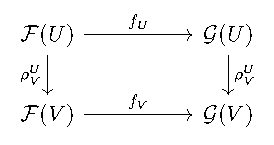
\includegraphics{lectures/7/pictures/cd_39.pdf}
		\end{center}
		коммутативны. 
	\end{definition}

	\begin{example}
		Приведём несколько примеров: 

		\begin{enumerate}
			\item Например, если у нас есть многообразие $M$, то  $\Omega^{\bullet}(\_)$ задаёт предпучок на нём. И, $C^{\infty}(\_)$ тоже. В принципе, всякие функции и формы~--- это основной пример. 

			\item \emph{Тривиальным предпучком} с группой $F$ называется предпучок $\cF$, сопоставляющий каждому открытому связному множеству группу $G$ и каждому вложению $V \hookrightarrow U$ тождественное отображение $G \to G$. 

			\item \emph{Постоянным предпучком} называется предпучок, изоморфный тривиальному. Предпучок называется \emph{локально постоянным}, если у каждой точки существует окрестность $U$ такая, что $\cF\vert_{U}$~--- постоянный предпучок. 

			\item \emph{Пучком} называется предпучок, удовлетворяющий \emph{условию склейки}, то есть $\forall U, V \subset X$, $\forall \sigma \in \cF(U), \ \tau \in \cF(V) \colon \sigma\vert_{U \cap V} = \tau\vert_{U \cap V}$ существует $\rho \in \cF(U \cup V)$ такой что $\rho\vert_{U} = \sigma$, $\rho\vert\_{V} = \tau$.

			Условие склейки вполне естественное. Как мы видели, оно выполняется, например, для дифференциальных форм.  

			\item Рассмотрим локально тривиальное расслоение $\pi \colon E \to M$. Тогда мы можем рассмотреть вот такой предпучок на $M$:
			\[
				\cH^{q}(U) \eqdef H^q(\pi^{-1}(U)).
			\]
			Если $U$~--- стягиваемое, из формулы Кюннета мы знаем, что 
			\[
				\cH^{q}(U) = H^q(U \times F) \cong H^q(F).
			\]

			Отсюда ясно, что если $M$~--- многообразие, то предпучок $\cH^{\bullet}$ является локально постоянным. 

			С другой стороны, если мы рассмотрим $E = M \times F$, то 
			\[
				\cH^{q}(M) = H^{q}(E) = \bigoplus_{i + j = n} H^i(M) \otimes H^{j}(F) 
			\]
			и обычно это не совпадает с $H^{q}(F)$. В общем, это мы всё к тому, что локально постоянный предпучок совсем не обязан быть постоянным. А вот локально постоянный пучок уже обязан быть постоянным. 
		\end{enumerate}

	\end{example}

	Перейдём к определению когомологий Чеха. 

	Пусть $X$~--- топологическое пространство, а $\fU = \{ U_{\alpha} \}_{\alpha}$~--- его открытое покрытие. 

	\begin{itemize}
		\item 0-коцепями на $X$ со значениями в предпучке $\cF$ называются функции, сопоставляющие каждому открытому множеству $U_{\alpha}$ элемент из $\cF(U_{\alpha})$, т.е. 
		\[
			C^{0}(\fU, \cF) = \prod_{\alpha \in \cJ} \cF(U_{\alpha}).
		\]
		\item Аналогично, 1-коцепями являются элементы 
		\[
			C^{1}(\fU, \cF) = \prod_{\alpha < \beta} \cF(U_{\alpha} \cap \cF_{\beta}).
		\]
		\item И так далее. $p$-коцепи определяются, как 
		\[
			C^{p}(\fU, \cF) = \prod_{\alpha_0 < \ldots < \alpha_p} \cF(U_{\alpha_0 \alpha_1 \ldots \alpha_p}).
		\]
	\end{itemize}

	Соответственно, последовательность вложений 
	\begin{center}
		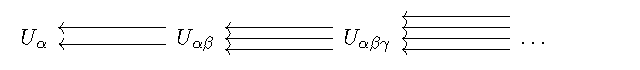
\includegraphics{lectures/7/pictures/cd_40.pdf}
	\end{center}
	индуцирует последовательность гомоморфизмов групп (ограничений)
	\begin{center}
		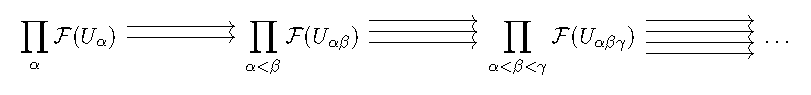
\includegraphics{lectures/7/pictures/cd_41.pdf}
	\end{center}

	Теперь определим дифференциал $\delta\colon C^{p}(\fU, \cF) \to C^{p}(\fU, \cF)$ как знакопеременную сумму ограничений, индуцированных вложениями $\delta_i\colon U_{\alpha_0, \ldots \alpha_{p + 1}} \to U_{\alpha_0, \ldots \alpha_{p}}$: 
	\[
		\delta = \cF(\partial_0) - \cF(\partial_1) + \ldots + (-1)^{p + 1} \cF(\partial_{p + 1}). 
	\]
	Или, можно еще в явном виде написать: 
	\[
		\omega \in C^{p}(\fU, \cF) = \prod_{\alpha_0 < \ldots < \alpha_p} \cF(U_{\alpha_0 \ldots \alpha_p}), \quad (\delta\omega)_{\alpha_0 \ldots \alpha_{p + 1}} = \sum_{i = 0}^{ p + 1 } (-1)^i \omega_{\alpha_0 \ldots \widehat{\alpha_i} \ldots \alpha_{p + 1}} . 
	\]

	\begin{remark}
		Под $\omega_{\alpha_0 \ldots \widehat{\alpha_i} \ldots \alpha_{p + 1}}$ мы подразумеваем сужение $\omega_{\alpha_0 \ldots \widehat{\alpha_i} \ldots \alpha_{p + 1}}$ на $U_{\alpha_0 \ldots \alpha_{p + 1}}$.
	\end{remark}

	\begin{lemma} 
		$\delta^2 = 0$.
	\end{lemma}
	\begin{proof}
		Полностью аналогично случаю комплекса Чеха-де Рама (да и в принципе всем таким доказательствам). 
	\end{proof}

	\begin{definition} 
		Соответственно, $(C^{\bullet}(\fU, \cF), \delta)$~--- коцепной комплекс. Его когомологии мы будем называть \emph{когомологиями Чеха} покрытия $\fU$ со значениями в $\cF$. Обозначать их мы будем, как $H^{\bullet}(\fU, \cF)$.   
	\end{definition}

	Обсудим, что произойдёт, если мы сменим покрытие. Напомним, что покрытие $\fV = \{ V_{\beta} \}_{\beta \in \cJ}$ называется \emph{измельчением} покрытия $\fU = \{ U_{\alpha} \}_{\alpha \in \cI}$, если существует такое отображение $\varphi\colon \cJ \to \cI$, что $V_{\beta} \subset U_{\varphi(\beta)}$. Соответственно, измельчение покрытия индуцирует отображение 
	\[
		\varphi^{\#} \colon C^{q}(\fU, \cF) \to C^{q}(\fV, \cF), \quad (\varphi^{\#} \omega)(V_{\beta_0 \ldots \beta_{q}}) = \omega(U_{\varphi_{\beta_0} \ldots \varphi(\beta_q)}). 
	\]

	\begin{lemma} 
		$\varphi^{\#}$~--- цепное отображение $C^{\bullet}(\fU, \cF) \to C^{\bullet}(\fV, \cF)$. 
	\end{lemma}

	\begin{proof}
		Нужно проверить, что оно коммутирует с дифференциалом, это стандартная простая выкладка. 
	\end{proof}

	\begin{lemma} 
		Пусть $\fU = \{ U_{\alpha} \}_{\alpha \in \cI}$~--- открытое покрытие, $\fV = \{ V_{\beta} \}_{\beta \in \cJ}$~--- его измельчение, а $\varphi, \psi \colon \cJ \to \cI$~--- два отображения измельчения. 

		Тогда  $\varphi^{\#}$ и $\psi^{\#}$ цепно гомотопны.
	\end{lemma}
	\begin{proof}
		Рассмотрим оператор $K\colon C^{q}(\fU, \cF) \to C^{q - 1}(\fU, \cF)$, определённый как 
		\[
			(K\omega)(V_{\beta_0 \ldots \beta_{q - 1}}) = \sum (-1)^i \omega(U_{\varphi(\beta_0) \varphi(\beta_i) \psi(\beta_i) \ldots \psi(\beta_{q - 1})}). 
		\]
		Покажем, что  $\psi^{\#} - \varphi^{\#} = \delta K + \delta K$. 
		\begin{center}
			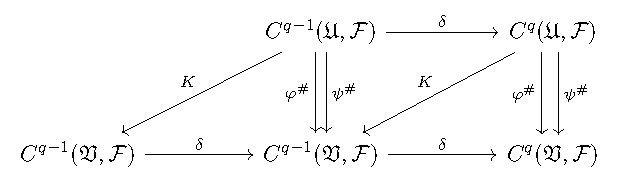
\includegraphics{lectures/7/pictures/cd_42.pdf}
		\end{center}

		В самом деле, 
		\begin{multline*}
			(K\delta \omega)(V_{\beta_0 \ldots \beta_{q - 1}}) = \sum (-1)^i (\delta \omega)(U_{\varphi(\beta_0) \ldots \varphi(\beta_i) \psi(\beta_i) \ldots \psi(\beta_{q - 1})}) = \\ = \sum_{i, j} (-1)^{i + j} \omega(U_{\varphi(\beta_0) \ldots \varphi(\beta_i) \psi(\beta_i) \ldots \psi(\beta_{q - 1})}) \text{ где пропущен } j \text{-й индекс}.
		\end{multline*}

		\begin{multline*}
			(\delta K \omega)(V_{\beta_0 \ldots \beta_{q - 1})}) = \sum (-1)^i (K \omega)(V_{\beta_{0} \ldots \widehat{\beta_i} \ldots \beta_{q  - 1}}) = \\ = \sum_{i, j} (-1)^{i + j} \omega(U_{\varphi_{(\beta_0) \ldots \varphi(\beta_j) \psi(\beta_j) \ldots \psi(\beta_{q - 1})}}) \text{ где пропущен } i \text{-й индекс}.
		\end{multline*}

		Как легко видеть, так как в первой сумме мы пропускаем $j$-й, а во втором $i$-й, каждое слагаемое $\omega(U_{\varphi(\beta_0) \ldots \varphi(\beta_j) \psi(\beta_j) \ldots \psi(\beta_{q - 1})})$ (кроме $i = j = 0$ и $i = j = q$) будет встречаться в первой и во второй сумме с разными знаками. Значит, останутся только 
		\[
			\omega(U_{\varphi(\beta_0) \ldots \varphi(\beta_{q - 1})}) - \omega(U_{\psi(\beta_0) \ldots \psi(\psi_{q - 1} ) }) = (\varphi^{\#}\omega)(V_{\beta_{0} \ldots \beta_{q - 1}}) - (\psi^{\#}\omega)(V_{\beta_{0} \ldots \beta_{q - 1} })
		\]

	\end{proof}

	Эта лемма нужна нам затем, чтобы при разных отображениях для одного и того же измельчения в когомологиях получалось одно и то же отображение. 

	Напомним, что набор $\{ G_{i} \}_{i \in \cI}$ называется \emph{индуктивной системой}, если при $\alpha > \beta$ у нас есть отображение $f_{\beta}^{\alpha}\colon G_{\alpha} \to G_{\beta}$ , причём 
	\begin{itemize}
		\item $f_{\alpha}^{\alpha} = \id$

		\item Если $\gamma < \beta < \alpha$, то $f_{\gamma}^{\alpha} = f_{\gamma}^{\beta} \circ f_{\beta}^{\alpha}$. 
	\end{itemize}

	Также напомним, что прямым пределом индуктивной системы групп называется 
	\[
		\varinjlim G_{i} = \prod_{i \in \cI} G_{i}/\sim,
	\]
	где $G_{\alpha} \ni a \sim b \in G_{\beta} \Leftrightarrow \exists \gamma\colon f_{\gamma}^{\alpha}(a) = f_{\gamma}^{\beta}(b)$.

	Ну или, проще говорить про универсальное свойство: 

	\begin{center}
		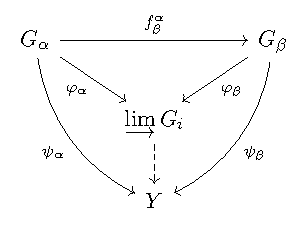
\includegraphics{lectures/7/pictures/cd_43.pdf}
	\end{center}

	Так вот, из доказанных выше двух лемм следует, что если $\fU > \fV$, то у нас есть корректно определённое отображение на когомологиях 
	\[
		H^{\bullet}(\fU, \cF) \to H^{\bullet}(\fV, \cF).
	\]
	Значит, $\{ H^{\bullet}(\fU, \cF) \}_{\fU}$~--- индуктивная система. Её прямой предел 
	\[
		H^{\bullet}(X, \cF) \eqdef \varinjlim H^{\bullet}(\fU, \cF)
	\]
	мы будем называть \emph{когомологиями Чеха пространства $X$ со значениями в предпучке $\cF$}.

	\begin{lemma} 
		Пусть $\R$~--- постоянный предпучок на многообразии $M$. Тогда 
		\[
			H^{q}(M, \R) \cong H^{q}_{\dR}(M).
		\]
	\end{lemma}
	\begin{proof}
		 Начнём с того, что хорошие покрытия образуют кофинальное подмножество в множестве всех покрытий\footnote{Подмножество $\cJ$ направленного множества $\cI$ называется кофинальным, если для любого $i \in I$ найдется $j \in \cJ$ такое что $i < j$}, поэтому мы можем рассматривать только хорошие покрытия. Для хороших покрытий мы доказывали, что $H^{\bullet}(\fU, \R) \cong H^{\bullet}_{\dR}(M)$. Но тогда ясно, что $H^{\bullet}(M, \R) \cong H^{\bullet}_{\dR}(M)$.                          
	\end{proof}

 


